\section{Transformer}

The Natural Language Processingcommunity once believed that Long Short-Term Memorys with attention could yield state-of-the-art performance on a variety of tasks. 

Long Short-Term Memorys and other Recurrent Neural Networks perform inference (and training) sequentially.
This sequential nature prevents parallelization at the sample level, limiting efficiency.
While parallelization can occur at the batch level, memory constraints restrict batching across too many examples.
These issues become particularly critical for long sequence lengths.

To overcome these bottlenecks, Google introduced the Transformer model, which replaces Recurrent Neural Networks with an attention mechanism. 
The key advantage of the Transformer is that it can perform operations in parallel, speeding up training.

In a Transformer, the encoder looks at all source tokens simultaneously. 
It processes each token iteratively in parallel, updating its representations over multiple layers.
The decoder, similarly, attends to both previous target tokens and source representations, updating its own state over multiple layers.

The Transformer architecture significantly reduces training time and allows for efficient parallelization across sequences.
\begin{figure}[H]
    \centering
    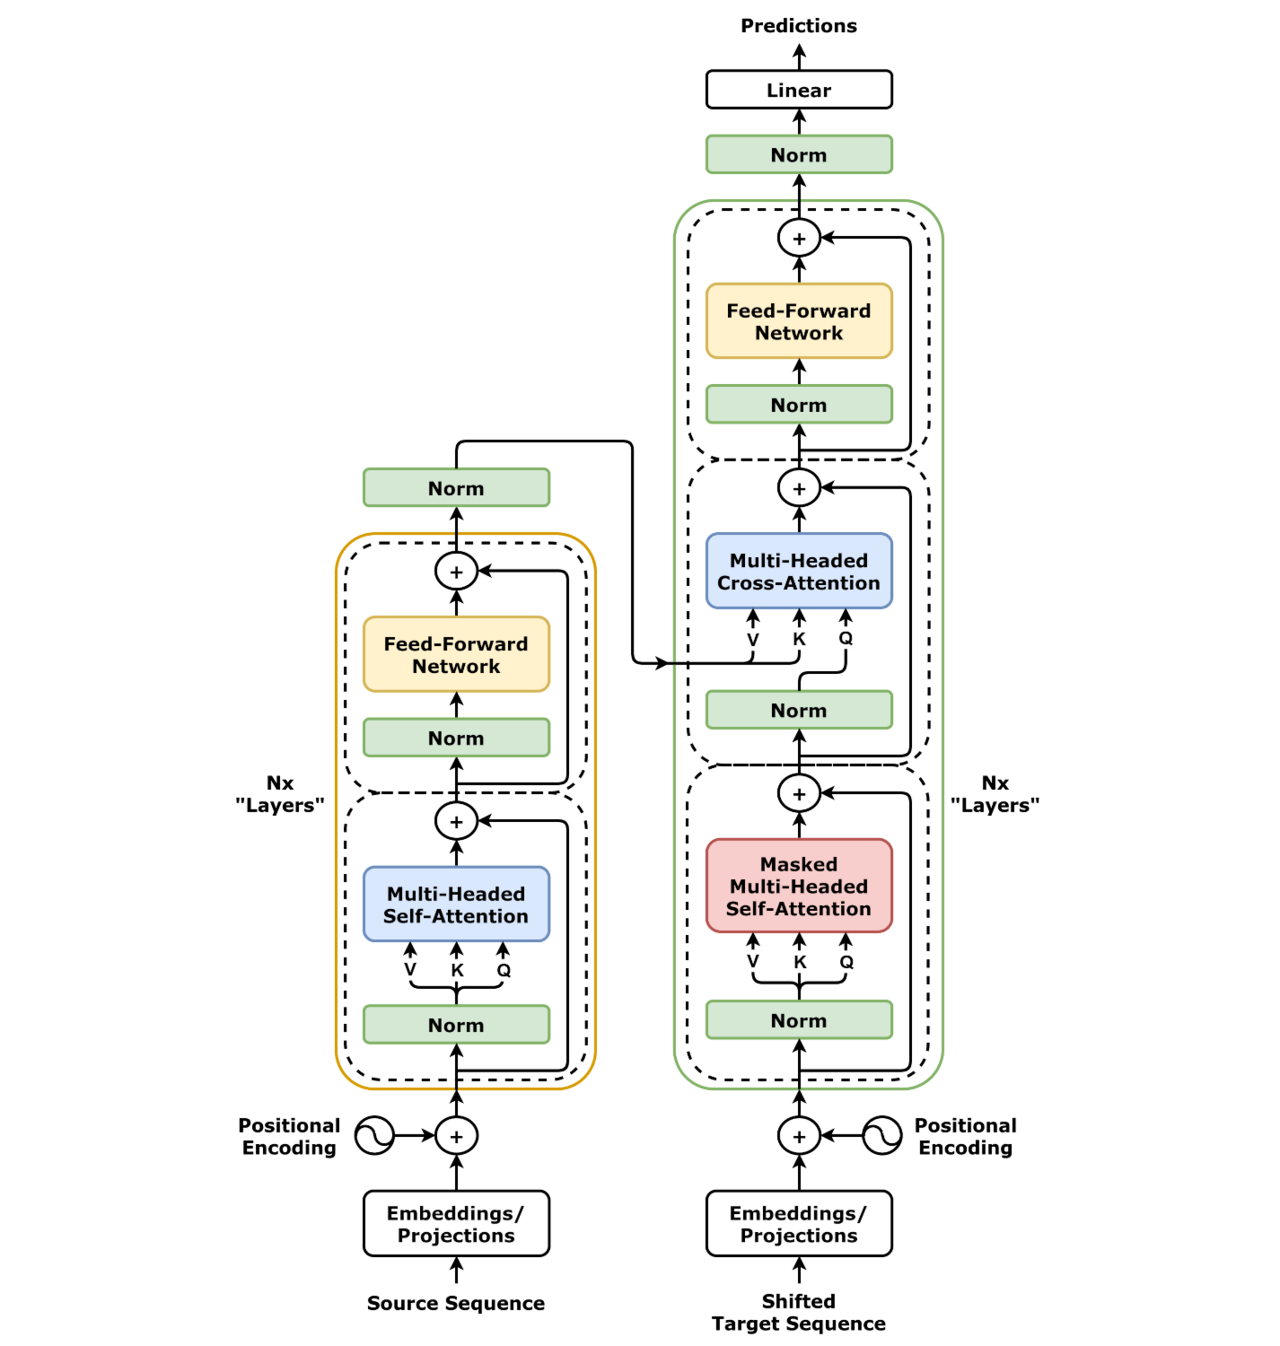
\includegraphics[width=0.75\linewidth]{images/trans.png}
    \caption{Transformer}
\end{figure}

\subsection{Encoder attention}
The encoder uses self-attention, where each token attends to all other tokens within the same input sequence. 
This is implemented using the following components:
\begin{itemize}
    \item \textit{Query}: a vector from which the attention mechanism queries information.
    \item \textit{Key}: a vector that the query looks at to compute weights for attention.
    \item \textit{Value}: the weighted sum of values is the attention output.
\end{itemize}
Self-attention allows for parallel execution and, consequently, parallel training, which helps improve training speed.

\paragraph*{Multi-head attention}
In some cases, attention needs to capture different aspects of a word's role in a sentence.
Multi-head attention enables the model to focus on multiple aspects simultaneously, both during encoding and decoding. 
This is achieved by concatenating several attention heads.
The use of multiple attention heads doesn't increase the model size, as the heads share the same model capacity.

\subsection{Decoder attention}
In the decoder, attention mechanisms differ during training and inference:
\begin{itemize}
    \item \textit{At inference time}: the decoder generates one token at a time since the sequence length is not known in advance, preventing any look-ahead.
    \item \textit{At training time}: the entire target sequence is known, allowing parallel processing of tokens but requiring the use of look-ahead masks to prevent the decoder from seeing future tokens during training.
\end{itemize}
While the training time complexity of Recurrent Neural Networks models is $\mathcal{O}(\text{len}(\text{source})+\text{len}(\text{target}))$, the Transformer achieves training in $\mathcal{O}(1)$ with respect to the length of fixed sequences, making it highly efficient.

\subsection{Other elements}
The other elements of the Transformer are: 
\begin{itemize}
    \item \textit{Decoder-encoder attention}: the decoder attends to the encoder states by using queries from the decoder and keys-values from the encoder states.
    \item \textit{Feed Forward Neural Networks}: after receiving attention-based information from other tokens, the model processes the information in feed-forward layers. 
        These are typically composed of two linear layers with ReLU activations.
        Residual connections are used to prevent issues like vanishing gradients and improve the flow of information.
    \item \textit{Layer normalization}: normalizes the representation of each vector independently within a batch, ensuring stable training.
        A scale and bias are applied globally across the layer and are trainable parameters.
\end{itemize}

\subsection{Positional encoding}
Since the Transformer model processes tokens in parallel, the order of tokens doesn't naturally affect the model's behavior, unlike Recurrent Neural Networks that process tokens sequentially. 
The self-attention mechanism is permutation-invariant, meaning changing the order of the tokens doesn't impact attention values.

To address this, positional encodings are added to the input embeddings to give the model information about the position of each token within the sequence. 
The input representation is the sum of:
\begin{itemize}
    \item \textit{Token embeddings}: standard word embeddings.
    \item \textit{Positional embeddings}: specific to each token's position in the sequence. 
\end{itemize}
Positional embeddings can be either learned or fixed. 
The original Transformer used fixed positional encodings, but modern state-of-the-art Transformers often learn these encodings to adapt more flexibly to varying sequence lengths